\section{Application}\label{sec:application}

\subsection{Data}

We apply the method to the motorway and A-road network of Great Britain. A site is a link of the Major Roads Database of the Department for Transport, a stretch of major road between two junctions with other major roads. For every link the annual average daily flow (AADF) is published each year by vehicle class, counted at the link in some years and estimated from earlier counts and regional traffic growth in others. Injury collisions reported to the police (STATS19) in 2015 to 2019 whose first road is a motorway or an A road were assigned to the nearest link carrying the same road number, provided they lay within 300\,m of the straight line joining the link's end nodes. Of 312{,}386 such collisions, 253{,}358 (81\%) were assigned. The others lie on links without a complete traffic series or further from the line. Links with an AADF in all five years were kept, which leaves 17{,}139 links and 85{,}695 link-years. All three sources are public, and the code that assembles the panel is part of the replication files.

Table~\ref{tab:uk-desc} describes the data. The average link is 2.8\,km long, carries about 21{,}600 motor vehicles a day and has 2.96 injury collisions a year, and 29\% of link-years have none. There are 15 candidate covariates. Six describe the traffic and vary by year: the logarithm of AADF, the shares of heavy goods vehicles, light goods vehicles, buses and coaches and motorcycles, and the logarithm of one plus the daily number of pedal cycles. Four describe the link and its surroundings and are constant over time: the logarithm of link length, a curvature index (the ratio of the link length along the road to the straight-line distance between its end nodes, on the log scale), the junction degree (the number of other major-road links meeting the link at its two ends) and the density of the major-road network within 2\,km of the link's midpoint, a proxy for urban settings. Five are binary: motorway, trunk A road (principal A roads are the reference), and London, Scotland and Wales, which differ in road administration and police reporting.

\begin{table}[!htbp]
\centering
\begin{threeparttable}
\caption{Descriptive statistics of the British major-road panel, 17{,}139 links observed from 2015 to 2019 (85{,}695 link-years).}
\label{tab:uk-desc}
\small
\setlength{\tabcolsep}{4pt}
\begin{tabular}{lrrrrr}
\toprule
Variable & Mean & SD & Min & Median & Max \\
\midrule
\tablerows{tables/uk_descriptives_rows.tex}
\bottomrule
\end{tabular}
\begin{tablenotes}\footnotesize
\item Shares are of all motor vehicles. Curvature index: link length along the road divided by the straight-line distance between the link's end nodes. Junction degree: number of other major-road links meeting the link at its two ends. Sources: STATS19 collisions, road traffic statistics (AADF) and the Major Roads Database, Department for Transport, Open Government Licence v3.0.
\end{tablenotes}
\end{threeparttable}
\end{table}

\subsection{Model setup}

The offset is the logarithm of link length, and the logarithm of AADF is a candidate, so its coefficient is the elasticity of the collision count with respect to traffic. Continuous candidates are winsorized at their 0.5th and 99.5th percentiles, centered and scaled to unit standard deviation (Remark~\ref{rem:centering}). We compare three versions of the proposed method, each with the random intercept of Section~\ref{sec:rpnb} as an additional candidate: M4 with a linear mean, M5 with the squares of the ten continuous candidates as fixed-only candidates, and M6, which adds dispersion selection with all 15 candidates as dispersion candidates. The conventional benchmark is M1, run with the constant as an additional candidate random parameter. The information criterion search M3 was not run, because at this sample size each of its several hundred simulated likelihood fits takes minutes.

The models are fitted to the four years 2015 to 2018 (68{,}556 link-years) and judged on the 2019 counts of the same links. The criterion is the log predictive density $\sum_i\log p(y_{i,2019}\mid\y_{\text{2015--18}})$, which conditions on everything the earlier years reveal about each link. For the proposed methods it is estimated by averaging the negative binomial probability of $y_{i,2019}$ over the posterior draws, including each link's draws $z_{ij}$. For M1 it averages over the Halton draws of each link, weighted by their likelihood for the link's 2015 to 2018 counts, which is the simulated posterior of the link's coefficients. Each proposed method is run as two chains of 3{,}000 iterations, of which the first 1{,}000 are discarded, with the default hyperparameters of Section~\ref{sec:prior}.

\subsection{Results}
\tbd{Results text from the long runs.}

\begin{table}[!htbp]
\centering
\begin{threeparttable}
\caption{Prediction of the 2019 collision counts of the 17{,}139 links from models fitted to 2015 to 2018.}
\label{tab:uk-predict}
\small
\setlength{\tabcolsep}{4pt}
\begin{tabular}{lcrrccr}
\toprule
Method & Random & LPD & $\Delta$LPD (SE) & MAE & RMSE & Minutes \\
\midrule
\tablerows{tables/uk_predict_rows.tex}
\bottomrule
\end{tabular}
\begin{tablenotes}\footnotesize
\item Random: number of covariates declared random (median probability rule for M4 to M6), and RI when the intercept is random. LPD: log predictive density of the 2019 counts, $\sum_i\log p(y_{i,2019}\mid\y_{\text{2015--18}})$, higher is better. $\Delta$LPD: difference from the best method, with the standard error of the sum of link-level differences. MAE and RMSE: mean absolute and root mean squared error of the predictive mean. Minutes: run time of one chain or of the full M1 procedure on one core. M1: sequential simulated maximum likelihood with a random constant. M4, M5 and M6: proposed method with a linear mean, a flexible mean, and a flexible mean with dispersion selection, each with a random intercept candidate.
\end{tablenotes}
\end{threeparttable}
\end{table}

\begin{figure}[!htbp]
\centering
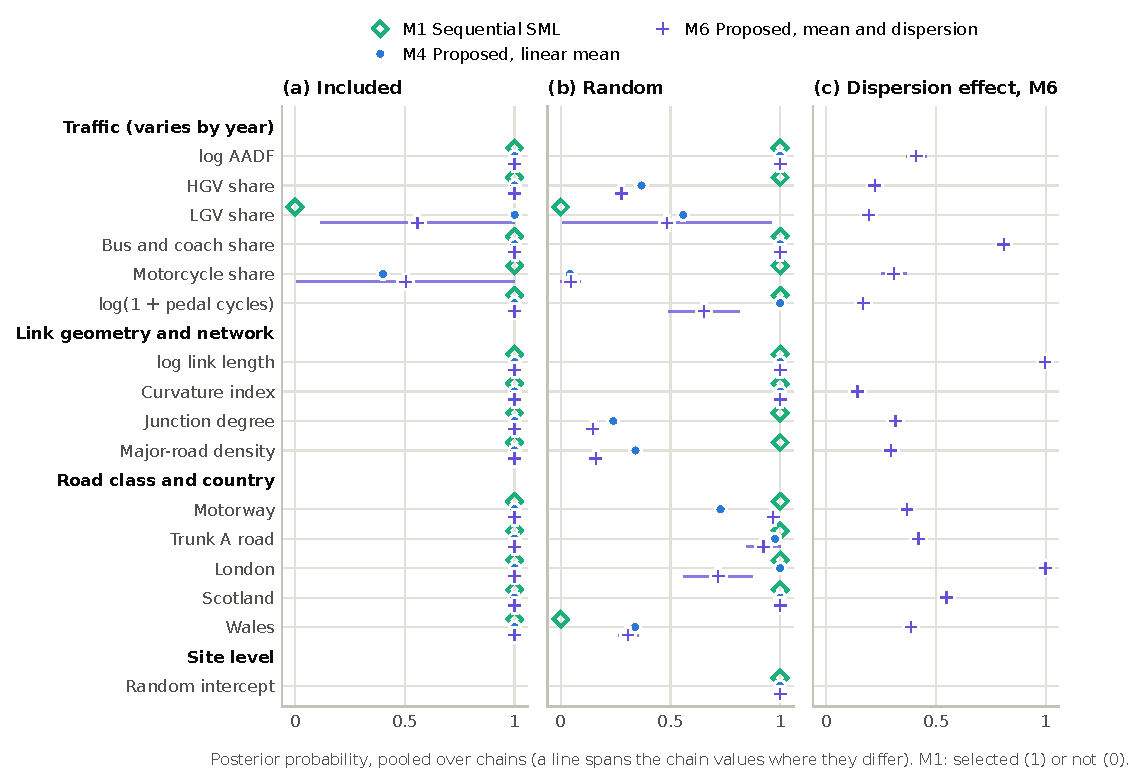
\includegraphics[width=\textwidth]{figures/uk_state_probabilities}
\caption{Specification of the British major-road model. (a) Posterior probability that a candidate is included, fixed or random. (b) Posterior probability that it is random. (c) Posterior probability that it affects the dispersion, under M6. Markers are pooled over chains, and a line spans the chain-specific values where they differ. For M1 the open diamond marks whether the candidate was selected (1) or not (0).}
\label{fig:uk-states}
\end{figure}

\begin{table}[!htbp]
\centering
\begin{threeparttable}
\caption{Model-averaged estimates from M6 for the British major-road links, 2015 to 2018. Continuous candidates are standardized, so coefficients are per standard deviation.}
\label{tab:uk-estimates}
\footnotesize
\setlength{\tabcolsep}{2pt}
\begin{tabular}{@{}lrcccccccc@{}}
\toprule
 & \multicolumn{2}{c}{Mean effect $\beta_j$} & & \multicolumn{2}{c}{Heterogeneity $|\sigma_j|$} & & & \multicolumn{2}{c}{Dispersion $\rho_k$} \\
\cmidrule(lr){2-3}\cmidrule(lr){5-6}\cmidrule(lr){9-10}
Candidate & Mean & 95\% interval & $P_j(\mathrm{R})$ & Mean & 95\% interval & Positive & $P_k(\mathrm{D})$ & Mean & 95\% interval \\
\midrule
\tablerows{tables/uk_estimates_rows.tex}
\bottomrule
\end{tabular}
\begin{tablenotes}\footnotesize
\item $\beta_j$: posterior mean and 95\% interval, averaged over specifications (zero when excluded). $|\sigma_j|$ and Positive (the share of links with a positive coefficient, $\Phi(\beta_j/|\sigma_j|)$) are given when $P_j(\mathrm{R})\ge0.5$, conditional on the parameter being random. $P_k(\mathrm{D})$: posterior probability of a dispersion effect, $\Pr(\eta_k=1\mid\y)$. $\rho_k$ is given when $P_k(\mathrm{D})\ge0.5$, conditional on inclusion. The dispersion is $r_{it}=\exp(\rho_0+\bm w_{it}^\top\bm\rho)$, so a positive $\rho_k$ means less overdispersion.
\end{tablenotes}
\end{threeparttable}
\end{table}

\subsection{Sensitivity}
\tbd{Results under $(a_\sigma,b_\sigma)\in\{(1,1),(1,4)\}$, $\tau_\sigma\in\{0.25,0.5,1\}$, and strong versus weak heredity.}
